\documentclass[tikz,border=3.14mm]{standalone}
\usetikzlibrary{calc,fadings,decorations.pathreplacing,decorations.markings,shadings}

\newcommand\pgfmathsinandcos[3]{%
    \pgfmathsetmacro#1{sin(#3)}%
    \pgfmathsetmacro#2{cos(#3)}%
}
\newcommand\LongitudePlane[3][current plane]{%
    \pgfmathsinandcos\sinEl\cosEl{#2} % elevation
    \pgfmathsinandcos\sint\cost{#3} % azimuth
    \tikzset{#1/.style={cm={\cost,\sint*\sinEl,0,\cosEl,(0,0)}}}
}

\newcommand\LatitudePlane[3][current plane]{%
    \pgfmathsinandcos\sinEl\cosEl{#2} % elevation
    \pgfmathsinandcos\sint\cost{#3} % latitude
    \pgfmathsetmacro\yshift{\RadiusSphere*\cosEl*\sint}
    \tikzset{#1/.style={cm={\cost,0,0,\cost*\sinEl,(0,\yshift)}}} %
}
\newcommand\NewLatitudePlane[4][current plane]{%
    \pgfmathsinandcos\sinEl\cosEl{#3} % elevation
    \pgfmathsinandcos\sint\cost{#4} % latitude
    \pgfmathsetmacro\yshift{#2*\cosEl*\sint}
    \tikzset{#1/.style={cm={\cost,0,0,\cost*\sinEl,(0,\yshift)}}} %
}
\newcommand\DrawLongitudeCircle[2][1]{
    \LongitudePlane{\angEl}{#2}
    \tikzset{current plane/.prefix style={scale=#1}}
    % angle of "visibility"
    \pgfmathsetmacro\angVis{atan(sin(#2)*cos(\angEl)/sin(\angEl))} %
    \draw[current plane] (\angVis:1) arc (\angVis:\angVis+180:1);
    \draw[current plane,opacity=0.4] (\angVis-180:1) arc (\angVis-180:\angVis:1);
}
\newcommand\DrawLongitudeArc[4][black]{
    \LongitudePlane{\angEl}{#2}
    \tikzset{current plane/.prefix style={scale=1}}
    \pgfmathsetmacro\angVis{atan(sin(#2)*cos(\angEl)/sin(\angEl))} %
    \pgfmathsetmacro\angA{mod(max(\angVis,#3),360)} %
    \pgfmathsetmacro\angB{mod(min(\angVis+180,#4),360} %
    \draw[current plane,#1,opacity=0.4] (#3:\RadiusSphere) arc (#3:#4:\RadiusSphere);
    \draw[current plane,#1]  (\angA:\RadiusSphere) arc (\angA:\angB:\RadiusSphere);
}%
\newcommand\DrawLatitudeCircle[2][1]{
    \LatitudePlane{\angEl}{#2}
    \tikzset{current plane/.prefix style={scale=#1}}
    \pgfmathsetmacro\sinVis{sin(#2)/cos(#2)*sin(\angEl)/cos(\angEl)}
    % angle of "visibility"
    \pgfmathsetmacro\angVis{asin(min(1,max(\sinVis,-1)))}
    \draw[current plane] (\angVis:1) arc (\angVis:-\angVis-180:1);
    \draw[current plane,opacity=0.4] (180-\angVis:1) arc (180-\angVis:\angVis:1);
}

\newcommand\DrawLatitudeArc[4][black]{
    \LatitudePlane{\angEl}{#2}
    \tikzset{current plane/.prefix style={scale=1}}
    \pgfmathsetmacro\sinVis{sin(#2)/cos(#2)*sin(\angEl)/cos(\angEl)}
    % angle of "visibility"
    \pgfmathsetmacro\angVis{asin(min(1,max(\sinVis,-1)))}
    \pgfmathsetmacro\angA{max(min(\angVis,#3),-\angVis-180)} %
    \pgfmathsetmacro\angB{min(\angVis,#4)} %
    \draw[current plane,#1,opacity=0.4] (#3:\RadiusSphere) arc (#3:#4:\RadiusSphere);
    \draw[current plane,#1] (\angA:\RadiusSphere) arc (\angA:\angB:\RadiusSphere);
}

%% document-wide tikz options and styles

\tikzset{%
    >=latex, % option for nice arrows
    inner sep=0pt,%
    outer sep=2pt,%
    mark coordinate/.style={inner sep=0pt,outer sep=0pt,minimum size=3pt,
        fill=black,circle}%
}

\begin{document}
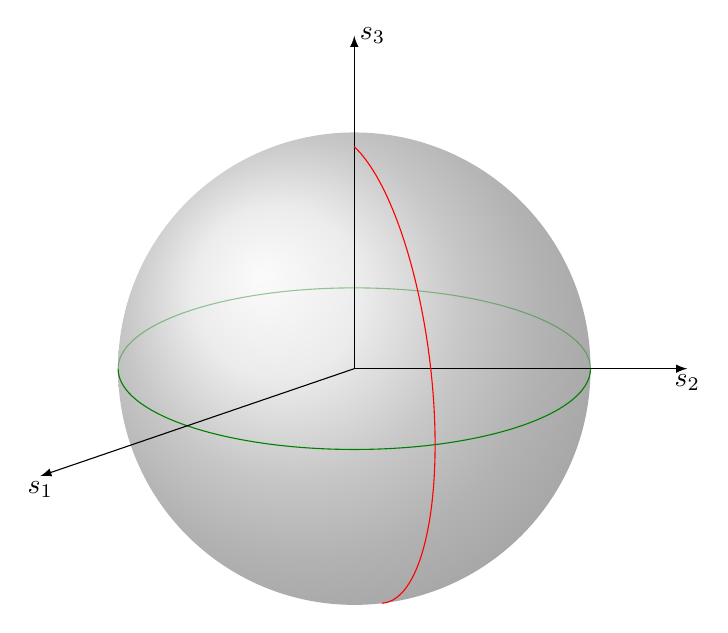
\begin{tikzpicture} % "THE GLOBE" showcase

    \def\RadiusSphere{3} % sphere radius
    \def\angEl{20} % elevation angle
    \def\angAz{-20} % azimuth angle
    
    \shade[ball color = gray!40, opacity = 0.5] (0,0) circle (\RadiusSphere);
    
    \pgfmathsetmacro\H{\RadiusSphere*cos(\angEl)} % distance to north pole
    \coordinate (O) at (0,0);
    %\node[circle,draw,black,scale=0.3] at (0,0) {};
    %\draw[right] node at (0,0){O};
    %\coordinate[mark coordinate] (N) at (0,\H);
    %\draw[left] node at (0,\H){N};
    %\coordinate[mark coordinate] (S) at (0,-\H);
    %\draw[left] node at (0,-\H){S};
    %\draw[thick, dashed, black](N)--(S);
    
    \tikzset{
        every path/.style={
            color=green!50!black
        }
    }
    \DrawLatitudeCircle[\RadiusSphere]{0}
    \tikzset{
        every path/.style={
            color=black
        }
    }
    
    
    \def\arcrad{2}
    \NewLatitudePlane[equator]{\RadiusSphere}{\angEl}{00};
    
    %\draw[-,dashed] (Oprime) -- (O) -- (Pprime);
    
    %%%%%%%%
    \def\angleLongitudeP{-110} % longitude of point P
    \def\angleLongitudeQ{-45} % longitude of point Q
    \def\angleLatitudeQ{30} % latitude  Q    ; 0 latitude of P 
    \def\angleLongitudeA{-20} % longitude of point A
    
    \LongitudePlane[PLongitudePlane]{\angleLongitudeP}{\angAz}
    \LongitudePlane[QLongitudePlane]{\angleLongitudeQ}{\angAz}
    \LongitudePlane[ALongitudePlane]{\angleLongitudeA}{\angAz}
    
    \path[ALongitudePlane] (32.5:\RadiusSphere) coordinate (A'); 
    \path[ALongitudePlane] (122.5:\RadiusSphere) coordinate (N'); 
    \path[PLongitudePlane] (00:\RadiusSphere) coordinate (P);
    
    \begin{scope}[x={(P)}, y={(A')}, z={(N')}]     
        %\draw[very thick,blue] (-135:0.75) arc (-135:45:0.75);
        %\draw[very thick,blue,-latex] (-135:0.75) arc (-135:-15:0.75);
        %\coordinate (Q) at (-60:0.75);
    \end{scope}
    
    %\draw (Q) -- (O);
    \path[equator] (135:{2*\RadiusSphere}) coordinate (X);
    \draw[-latex] (O) -- (X) node[below]{$s_1$};
    \path[equator] (0:{1.5*\RadiusSphere}) coordinate (Y);
    \draw[-latex] (O) -- (Y) node[below]{$s_2$};
    \draw[-latex] (O)-- (0,1.5*\H) node[right]{$s_3$};
    
    \LongitudePlane[angle]{\angEl}{-70};
    \draw[angle,-,red] (-70:\RadiusSphere) arc (-70:90:\RadiusSphere);
    
    %\draw[equator,-,red] (135:\arcrad) arc (135:100:\arcrad) node[pos=0.7,above]{$\Omega$};

\end{tikzpicture}
\end{document}